\chapter{Cơ Sở Lý Thuyết Và Các Nghiên Cứu Liên Quan}
\ifpdf
    \graphicspath{{Chapter2/Chapter2Figs/PNG/}{Chapter2/Chapter2Figs/PDF/}{Chapter2/Chapter2Figs/}}
\else
    \graphicspath{{Chapter2/Chapter2Figs/EPS/}{Chapter2/Chapter2Figs/}}
\fi

Chương này tập trung vào việc tìm hiểu tổng quan bài toán mô tả hình ảnh và các phương pháp được áp dụng trên các tập dữ liệu lớn như Faster R-CNN \cite{ren2015faster} và YOLOv7 \cite{wang2022yolov7}.

\section{Tổng quan về bài toán nhận diện vật thể}
\markboth{\MakeUppercase{\thechapter. Cơ Sở Cơ Sở Lý Thuyết Và Các Nghiên Cứu Liên Quan}}{\thechapter. Cơ Sở Cơ Sở Lý Thuyết Và Các Nghiên Cứu Liên Quan}
Bài toán nhận diện vật thể (object detection) là một trong những bài toán quan trọng của lĩnh vực Computer Vision. Bài toán này yêu cầu máy tính phải nhận dạng các đối tượng (thuộc về một lớp cụ thể như con người, xe, máy tính…) trong ảnh hoặc video, đồng thời xác định vị trí của những đối tượng này trong bức ảnh (video) đó. Mục tiêu của bài toán nhận diện vật thể chính là mô phỏng khả năng thị giác của con người vào máy tính.

Trong khi số lượng các loại vật thể trong một bức ảnh không nhiều, nhận diện vật thể được đánh giá là bài toán có tính thách thức cao bởi số lượng lớn các khả năng về vị trí cũng như kích thước của các đối tượng. Do đó, bài toán nhận diện vật thể vẫn luôn là một lĩnh vực cần được nhiều sự nghiên cứu.

Hiện nay, có rất nhiều phương pháp để giải quyết bài toán nhận diện vật thể, tùy vào tính chất và độ phức tạp của bài toán mà mỗi phương pháp có ưu, nhược điểm khác nhau. Bao gồm các phương pháp truyền thống dựa trên sự phân tích và rút trích đặc trưng như Haar Cascades, Viola-Jones… và các phương pháp hiện đại sử dụng thuật toán Deep Learning như SSD, Faster R-CNN, YOLO... Thông thường, các thuật toán Deep Learning cho ra kết quả tốt hơn so với các phương pháp cổ điển, đặc biệt là khi xử lý các vật thể phức tạp và có nhiều biến thể khác nhau.

\begin{figure}[h!]
	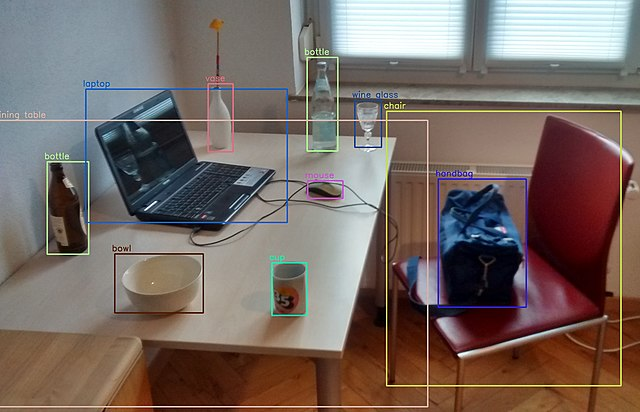
\includegraphics[width=\textwidth]{Detected-with-YOLO--Schreibtisch-mit-Objekten.jpg}
	\caption{Nhận diện các vật thể trong một căn phòng}
\end{figure}

Các phương pháp sử dụng Deep Learning cho bài toán nhận diện vật thể có thể được chia thành hai loại chính: two-stages và one-stage \cite{Deng2020}. Trong two-stage, mô hình sẽ đưa ra các vùng tiềm năng chứa đối tượng trước khi xác định đối tượng. Ví dụ như phương pháp Faster R-CNN sẽ sử dụng Region Proposal Network (RPN) để đưa ra các vùng tiềm năng trước khi đưa vào mô hình để xác định đối tượng. Ngược lại, trong one-stage, mô hình sẽ trực tiếp dự đoán các bounding box và loại đối tượng tương ứng trong ảnh. Tiêu biểu của one-stage là phương pháp YOLO (You Only Look Once) sẽ trực tiếp dự đoán bounding box và loại đối tượng trong ảnh.

Tuy nhiên, bài toán nhận diện vật thể vẫn còn rất nhiều thách thức, đặc biệt là khi đối tượng có kích thước nhỏ, có nhiều biến thể hoặc ở nhiều vị trí khác nhau trên ảnh. Để giải quyết những thách thức này, bài toán vẫn cần được nghiên cứu và đưa ra những giải pháp mới tối ưu hơn.



Tóm lại, bài toán nhận diện vật thể là một bài toán quan trọng trong lĩnh vực Computer Vision. Có nhiều phương pháp để giải quyết bài toán này, từ các phương pháp cổ điển đến các phương pháp sử dụng Deep Learning. Tuy nhiên, bài toán vẫn còn nhiều thách thức và cần nghiên cứu thêm để giải quyết.


\section{Faster R-CNN}
\markboth{\MakeUppercase{\thechapter. Cơ Sở Lý Thuyết Và Các Nghiên Cứu Liên Quan }}{\thechapter. Cơ Sở Lý Thuyết Và Các Nghiên Cứu Liên Quan}

Faster R-CNN (Region-based Convolutional Neural Network) là một mô hình deep learning được phát triển để giải quyết bài toán Object Detection - phát hiện và nhận diện vật thể. Với tốc độ và sự chính xác của mình, mô hình Faster R-CNN đã trở thành một trong những giải pháp tiên tiến nhất hiện nay trong lĩnh vực này. Để thực sự hiểu về Faster R-CNN, trước tiên chúng ta cần tìm hiểu ngắn gọn về kiến trúc chung và các tiền thân của nó, đó là R-CNN và Fast R-CNN.

\subsection{Kiến trúc chung}
Các mô hình họ R-CNN tương tự như các kỹ thuật nhận diện vật thể truyền thống, được thực hiện thông qua 3 bước chính: Tạo các vùng đề xuất hình ảnh (Region proposals generator), trích lọc đặc trưng (Feature extraction) và phân loại đối tượng (Classification). 

\begin{figure}
	\centering
	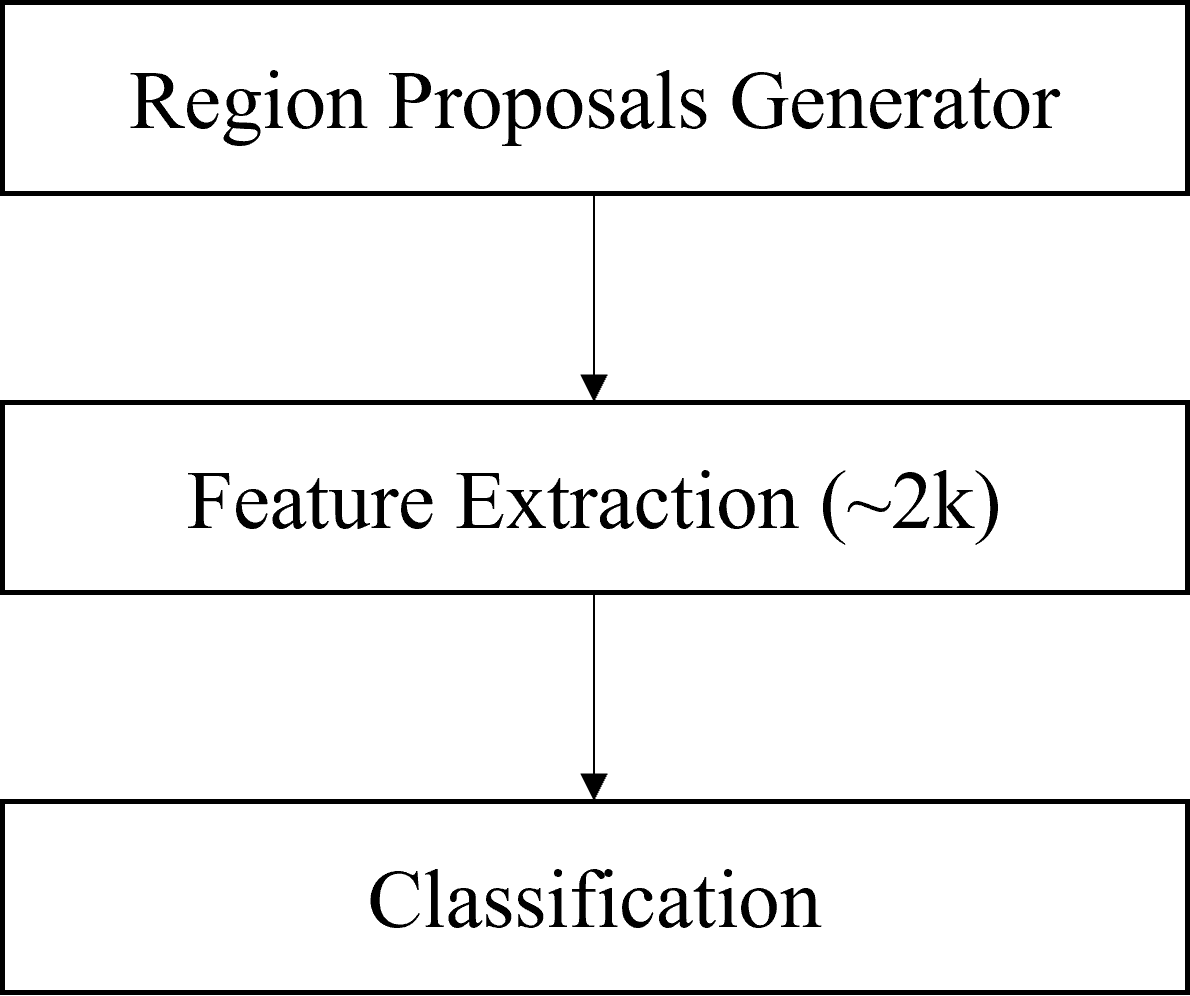
\includegraphics[scale=1]{Traditional-object-detecton-pipeline.png}
	\caption{Object detection pipeline}
	\label{fig:OD-pipeline}
\end{figure}

\nomenclature{Pipeline}{Tập hợp các bước xử lý liên tiếp nhận đầu vào là dữ liệu (ảnh, âm thanh, các trường dữ liệu) và trả ra kết quả dự doán ở output.}

Bước đầu tiên của quy trình có tác dụng tạo và trích xuất các vùng có thể chứa vật thể được bao bởi các bounding box. Các region proposal là các vùng có khả năng chứa các đối tượng hoặc hình ảnh ở bên trong đó. Số lượng các region proposal này thường rất lớn (khoảng 2 ngàn hoặc hơn). Một số thuật toán tạo ra các region proposal có thể kể đến là Selective Search và EdgeBoxes.

\nomenclature{Region proposal}{Vùng đề xuất, là những vùng mà có khả năng chứa đối tượng ở bên trong nó.}
\nomenclature{Bounding box}{Hình chữ nhật được vẽ bao quan đối tượng nhằm xác định đối tượng.}

Với mỗi region proposal, một vector đặc trưng có độ dài cố định được trích xuất bằng cách sử dụng các mô tả đặc trưng hình ảnh khác nhau, ví dụ như Histogram of Oriented Gradients (HOG). Vector đặc trưng này rất quan trọng đối với thành công của mô hình nhận diện vật thể. Do đó, một vector đặc trưng cần phải mô tả đủ đối tượng ngay cả khi đối tượng bị thay đổi về tỉ lệ hay ở một vị trí khác.

Các vector đặc trưng sau đó được sử dụng để gán từng region proposal vào lớp nền hoặc một trong các lớp đối tượng. Khi số lượng lớp tăng lên, độ phức tạp của việc xây dựng mô hình nhằm phân biệt giữa các đối tượng này cũng tăng lên. Một thuật toán phổ biến được dùng để tách các đối tượng khác nhau vào đúng lớp là Support Vector Machine (SVM).


\subsection{R-CNN (2014)}
R-CNN (Region-based Convolutional Neural Networks) là một mô hình mạng neural sử dụng cho bài toán nhận dạng vật thể trong hình ảnh \cite{girshick2014rich}. Được giới thiệu lần đầu tiên vào năm 2014 bởi Ross Girshick, Jeff Donahue, Trevor Darrell và Jitendra Malik, R-CNN đã tạo ra một bước đột phá trong việc giải quyết bài toán nhận dạng vật thể trong hình ảnh.

Bước đầu tiên trong pipeline của R-CNN nhằm sinh ra các region proposal dựa trên thuật toán selective search \cite{uijlings2013selective}. Thuật toán selective search tạo ra các vùng phân đoạn phụ (sub-segmentation) từ hình ảnh có thể thuộc về một đối tượng (dựa trên các đặc trưng màu sắc, kích thước, hình dạng hay kết cấu) và lặp lại việc kết hợp các vùng giống nhau để tạo nên các đối tượng.

\begin{figure}[h]
	\centering
	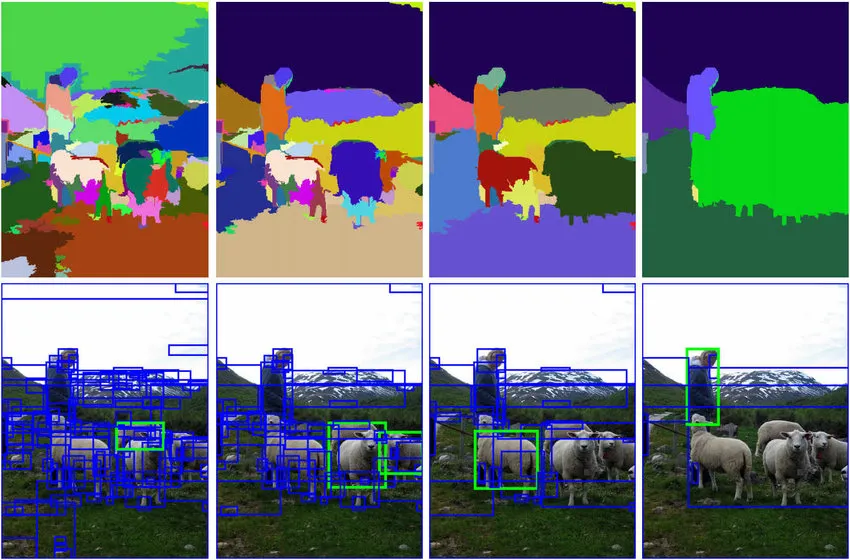
\includegraphics[scale=0.4]{Example-selective-search.png}
	\caption{Hình ảnh minh họa về thuật toán Selective search}
\end{figure}

Đóng góp chính của R-CNN vào quy trình chung (Hình \ref{fig:OD-pipeline}) chỉ đơn giản là thực hiện trích xuất đặc trưng dựa trên một mạng CNN học sâu. Các region proposal đã tạo ra sau đó được điều chỉnh về một kích thước cố định (4,096). Cuối cùng, mô hình sử dụng thuật toán pre-trained SVM nhằm phân loại các đối tượng trong các vùng ảnh đó.

\begin{figure}[h]
	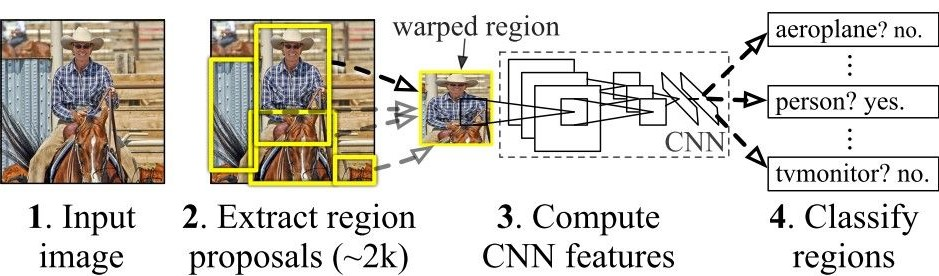
\includegraphics[width=\textwidth]{RCNN-overview.jpg}
	\caption{Hình ảnh minh họa kiến trúc R-CNN \textmd{(được trích xuất từ bài báo gốc \cite{girshick2014rich}). Mô hình (1) đọc ảnh đầu vào, (2) trích xuất khoảng 2000 region proposal, (3) tính toán các đặc trưng trên từng đề xuất bằng CNN, cuối cùng (4) phân lớp từng khu vực sử dụng SVMs. }}
\end{figure}

R-CNN là một trong những mô hình đầu tiên sử dụng mạng học sâu để nhận diện vật thể trên hình ảnh. Việc kết hợp các phương pháp truyền thống và mạng học sâu là một bước đột phá trong bài toán nhận diện vật thể, mô hình đã cho thấy khả năng phát hiện và nhận dạng vật thể với độ chính xác cao hơn so với phương pháp truyền thống (khoảng 30\% so với kết quả tốt nhất trước đó trên PASCAL VOC 2012 \citep{girshick2014rich}). Không những thế, nhờ sự ứng dụng CNN tương đối đơn giản và dễ hiểu, mô hình R-CNN còn cho thấy khả năng mở rộng số lượng các lớp của mình. 


Mặc dù R-CNN đã đem đến nhiều ưu điểm và đột phá trong việc phát hiện và nhận dạng vật thể, nhưng mô hình này cũng tồn tại nhiều hạn chế. Trong đó, đáng nói nhất là tốc độ xử lý chậm, đặc biệt là trong quá trình tạo các region proposals và trích xuất đặc trưng. Mỗi region proposal trong khoảng 2000 vùng được selective search tạo ra phải được đưa vào mạng CNN độc lập với nhau, đồng nghĩa với việc có khoảng 2000 vùng ảnh phải đi qua CNN, do đó quá trình này cần một khoảng thời gian rất lớn, nhận dạng trên tập VGG16 cần 47s / ảnh (GPU) \citep{girshick2014rich}, làm cho việc chạy R-CNN trong thời gian thực (real-time) là bất khả thi. Không những thế, mô hình R-CNN cần lưu lại các đặc trưng đã được trích xuất từ mạng CNN để huấn luyện SVMs sau đó, dẫn đến việc mô hình yêu cầu một tài nguyên bộ nhớ đáng kể. 

Để giải quyết được những nhược điểm trên, Fast R-CNN \cite{Girshick_2015_ICCV} đã được ra đời nhằm khắc phục những hạn chế, đồng thời cải thiện các ưu điểm của R-CNN.

\subsection{Fast R-CNN (2015)} 
Fast R-CNN là một mô hình phát hiện đối tượng trong Computer Vision, được giới thiệu bởi Ross Girshick vào năm 2015 \citep{Girshick_2015_ICCV}. Fast R-CNN được xây dựng dựa trên mô hình R-CNN trước đó nhằm phân loại hiệu quả các region proposals bằng cách sử dụng mạng CNN. So với R-CNN, Fast R-CNN đã có nhiều cải tiến nhằm cải thiện tốc độ huấn luyện và kiểm tra, trong khi vẫn tăng độ chính xác. Fast R-CNN huấn luyện trên mạng VGG16 nhanh hơn R-CNN gấp 9 lần, trong khi cho ra kết quả nhanh hơn 213 lần tại thời điểm thử nghiệm (test-time) và đạt được mAP cao hơn trên PASCAL VOC 2012 với mAP khoảng 66\% (vs. 62\% sử dụng R-CNN).

\nomenclature{mAP}{mean Average Precision}

\begin{figure}
	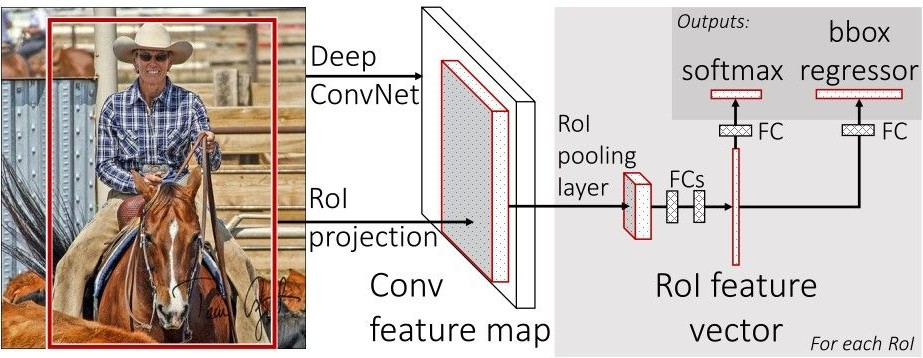
\includegraphics[width=\textwidth]{Fast-RCNN-overview.jpg}
	\caption{Kiến trúc của Fast R-CNN}
	\label{fig:Fast-RCNN-Architecture}
\end{figure}

Hình \ref{fig:Fast-RCNN-Architecture} thể hiện cách Fast R-CNN tiếp cận bài toán nhận diện vật thể theo tương tự như R-CNN. Tuy nhiên, thay vì đưa từng region proposals vào CNN, Fast R-CNN đưa cả bức ảnh vào ConvNet nhằm tạo một conv feature map. Từ conv feature map, mô hình xác định các region proposals, sau đó nén chúng thành các hình vuông có kích thước cố định (định nghĩa trước) bằng cách sử dụng RoI Pooling. Các vector đặc trưng được đưa vào Fully connected layer bao gồm 1 lớp softmax dự đoán lớp cho các region proposals và giá trị offset của bounding box thông qua bbox regressor. 

\nomenclature{RoI}{Region of Interest}

\begin{figure}[h]
	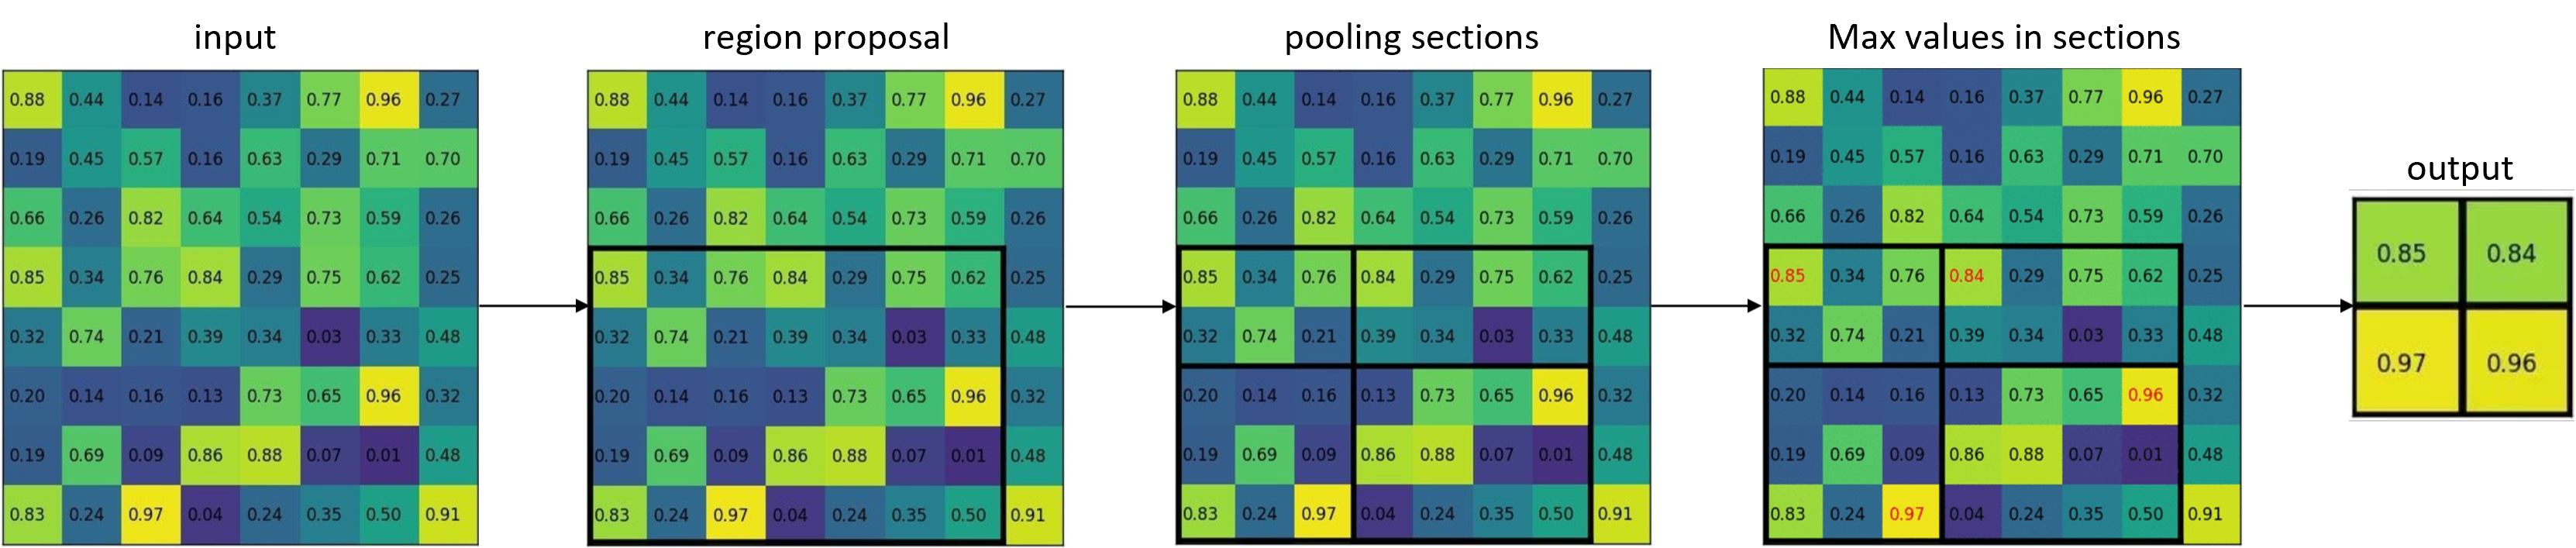
\includegraphics[width=\textwidth]{RoI-Pooling-example.png}
	\caption{Hình ảnh minh họa RoI Pooling}
\end{figure}

Bằng việc tạo conv feature map bằng ConvNet, Fast R-CNN đã tránh được việc phải đưa 2000 region proposals vào mạng CNN với mỗi ảnh. Thay vào đó, mô hình chỉ thực hiện trích xuất đặc trưng một lần mỗi ảnh, sau đó tạo ra một conv feature map dùng chung cho input. Từ đó, tăng tốc độ xử lý của Fast R-CNN một cách đáng kể so với R-CNN. Tuy nhiên, việc yêu cầu các region proposal của thuật toán làm giảm tốc độ xử lý so với trường hợp không sử dụng chúng. Do đó, region proposals trở thành một trong những hạn chế, ảnh hưởng đến hiệu suất trong cả mô hình Fast R-CNN và R-CNN. 


\subsection{Faster R-CNN (2016)}
Các mạng nhận diện vật thể dựa trên thuật toán region proposals nhằm giả định vị trí của các đối tượng. Các thuật toán như SPPnet \cite{he2015spatial} và Fast R-CNN \cite{Girshick_2015_ICCV} đã giảm thời gian xử lý của các mạng nhận diện này, tuy nhiên vẫn chia sẻ chung một điểm hạn chế trong quá trình tính toán các region proposals. Để khắc phục hạn chế này, vào năm 2015, Shaoquing Ren cùng nhóm nghiên cứu của mình trong bài báo về Faster R-CNN \citep{ren2015faster} đã giới thiệu \textit{Region Proposal Network} (RPN), qua đó giảm thiểu chi phí cần cho việc tính toán region proposals gần như bằng không. Faster R-CNN tốt hơn hẳn Fast R-CNN cả về tốc độ lẫn độ chính xác.

Những đóng góp chính trong bài báo này \citep{ren2015faster} bao gồm:
\begin{enumerate}
	\itemsep0em
	\item Sử dụng \textbf{region proposal network (RPN)}, một mạng tích chập toàn phần (Fully convolutional network) sinh ra các vùng đề xuất với các scale và aspect ratio khác nhau. Mạng RPN triển khai thuật ngữ neural network with attention nhằm hướng Fast R-CNN vị trí cần xử lý.
	\item Đề xuất một khái niệm mới thay thế cho việc sử dụng \textbf{pyramids of images} (nhiều thể hiện có kích thước khác nhau của cùng một ảnh số) và \textbf{pyramids of filters} (nhiều filters với kích thước khác nhau), đó là \textbf{anchor boxes}. Mỗi vùng đề xuất được ánh xạ đến từng anchor box tương ứng, sau đó nhận diện các vật thể với các scale và aspect ratio khác nhau.
	\item Tối ưu hóa xen kẽ, cho phép RPN và Fast R-CNN huấn luyện trên cùng một conv features. Qua đó làm giảm đáng kể thời gian tính toán.
\end{enumerate}

\nomenclature{Scale}{Độ phóng đại so với khung hình gốc}
\nomenclature{Aspect ratio}{Tỷ lệ cạnh $w/h$}

%18:39 04/26/2023

\begin{figure}[h]
	\center
	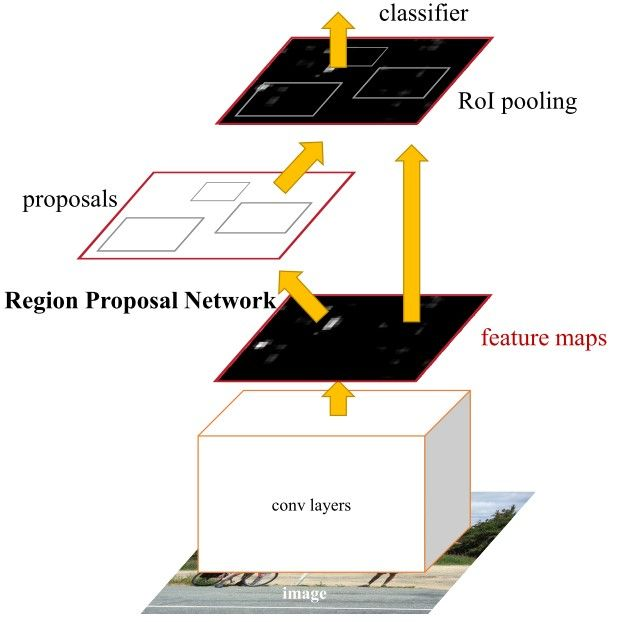
\includegraphics[scale=0.45]{Faster-RCNN-architecture.jpg}
	\caption{Kiến trúc của Faster R-CNN \textmd{}}
	\label{fig:faster-rcnn-architecture}
\end{figure}

Kiến trúc của Faster R-CNN được thể hiện như hình \ref{fig:faster-rcnn-architecture}, bao gồm 2 module là \textbf{RPN} (tạo các region proposals) và \textbf{Fast R-CNN} (phát hiện các đối tượng trong region proposals). Conv feature maps được sử dụng chung cho cả hai module. Mô hình Faster R-CNN thực hiện xử lý theo các bước sau:

\begin{itemize}
	\itemsep0em
	\item RPN tạo ra các region proposals.
	\item Với mỗi region proposal trong ảnh, một vector đặc trưng có độ dài cố định được trích xuất sử dụng một lớp RoI Pooling.
	\item Các vector đặc trưng trên được phân lớp bằng module Fast R-CNN.
	\item Trả về bounding-boxes kèm theo scores của các đối tượng được nhận diện.
\end{itemize}

\subsubsection*{Region Proposal Network}
Một mạng RPN (Region Proposal Network) nhận một ảnh (có kích thước bất kỳ) làm đầu vào và đưa ra một tập hợp các đề xuất vật thể được chứa trong hình chữ nhật, mỗi đề xuất được gán một \nameref{obj-score}. Quá trình này được mô hình hóa bằng một mạng tích chập toàn phần.

Nhằm tạo ra các region proposals, một mạng nhỏ được sử dụng để trượt trên conv feature map (hình \ref{fig:RPN-architecture}). Mạng này được kết nối đầy đủ với một cửa sổ không gian $n \times n$ của conv feature map đầu vào. Mỗi cửa sổ trượt được ánh xạ thành một vector có số chiều ít hơn (256-d đối với ZF và 512-d đối với VGG). Một cửa sổ trượt có thể tạo ra rất nhiều region proposals. Tuy nhiên, các region proposals này không được đưa vào các mạng hồi quy và phân lớp ngay lập tức mà được loại bỏ bớt dựa trên "objectness score".

\subsubsection*{Translation-Invariant Anchors}
Kết quả của quá trình trên, mô hình đưa ra đồng thời $k$ region proposals, do đó lớp $reg$ có $4k$ đầu ra nhằm mã hóa tọa độ của $k$ đề xuất. Trong khi lớp $cls$ có $2k$ đầu ra nhằm ước tính xác suất là vật thể hay không phải vật thể với mỗi đề xuất. Mỗi đề xuất được tham số hóa theo một hộp tham chiếu, gọi là $anchor$ $ box$. Các anchor được căn chỉnh ở chính giữa tại cửa sổ trượt tương ứng, và bao gồm 2 tham số là \textit{Scale} và \textit{Aspect ratio}. Số lượng scale và aspect ratio thường được chọn bằng 3, cho ra $k=9$ anchors (multi-scale anchors) tại mỗi vị trí trượt.
Đối với một feature map có kích thước $W \times H$ ($\sim$ 2,400), thuật toán sẽ đưa ra tổng cộng $W H k$ anchors.

%\vspace{.5cm}
\begin{figure}[h]
	\center
	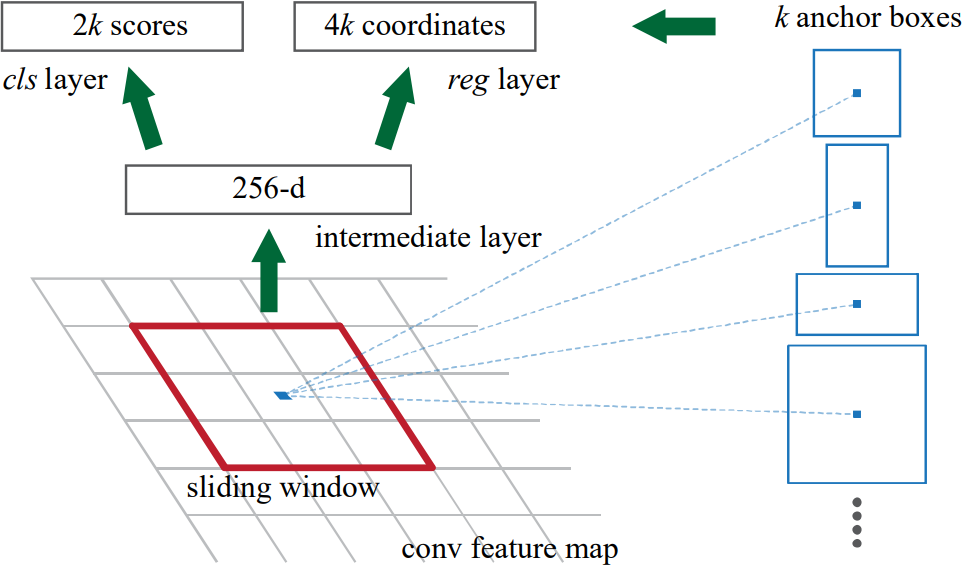
\includegraphics[scale=.5]{RPN-architecture.png}
	\caption{Hình ảnh minh họa kiến trúc RPN \textmd{(ảnh trích xuất từ bài báo Ren et al. \citep{ren2015faster})}}
	\label{fig:RPN-architecture}
\end{figure}

Việc sử dụng các anchor boxes làm cho mô hình có thể có được scale-invariant (thuộc tính mô hình không thay đổi khi kích thước của vật thể thay đổi) và translation-invariant (thuộc tính mô hình không thay đổi khi vị trí của vật thể thay đổi), trong khi chỉ yêu cầu 1 ảnh số với 1 kích thước duy nhất. Điều này giúp cho mô hình tránh phải sử dụng nhiều ảnh số hay nhiều filters. Các multi-scale anchors là điều kiện thiết yếu giúp chia sẻ các đặc trưng giữa RPN và mạng Fast R-CNN, qua đó giảm thiểu số lượng tham số và thời gian xử lý.

\subsubsection*{Object Score}
\label{obj-score}
Với mỗi anchor, lớp $cls$ trả về một vector có độ dài 2 thể hiện việc là vật thể hoặc không chứa vật thể (background) của anchor đó. Nếu vector trả về có giá trị [1, 0], thì anchor đang xét được phân loại là background. Ngược lại, nếu vector trả về có giá trị [0, 1], anchor đó có chứa vật thể.

Để huấn luyện mạng RPNs, mỗi anchors được gán một nhãn nhị phân (là vật thể hoặc không là vật thể). Các nhãn positive hoặc negative được gán cho anchors dựa trên một độ đo gọi là Intersection-over-Union (IoU).

IoU đo lường tỉ lệ giữa diện tích phần giao giữa 2 vùng quan tâm (region of interest, RoIs) và diện tích phần hợp của chúng. Giá trị của IoU nằm trong khoảng từ 0.0 đến 1.0. Khi 2 RoIs không giao nhau, IoU nhận giá trị là 0.0. Ngược lại, IoU bằng 1.0 khi 2 RoIs hoàn toàn trùng khớp với nhau. Cụ thể, trong quá trình huấn luyện RPNs, IoU được tính giữa các anchors và các ground-truth box.

Dựa trên IoU giữa anchor box và ground-truth box, RPN có thể quyết định objectness score cho từng anchor box theo các quy tắc sau: (i) Anchor box có IoU lớn hơn 0.7 với bất kỳ ground-truth box nào có objectness score là positive, (ii) nếu không anchor nào có IoU lớn hơn 0.7, nhãn positive được gán cho anchor(s) có IoU cao nhất với một ground-truth box bất kỳ, (iii) một anchor có objectness score là negative nếu IoU trên tất cả các ground-truth box nhỏ hơn 0.3 và (iv) các anchor có objectness score không phải là positive hay negative không ảnh hưởng đến tính khách quan của quá trình huấn luyện.

Objectness score có thể được tổng quát bằng công thức sau:
\begin{equation}
	\begin{split}
	Objectness\_score(Io&U) = \begin{cases}
								positive, & IoU > 0.7 \\
								negative, & IoU < 0.3 \\
								just\_ignore, & otherwise 
							\end{cases} \\
	&\textit{With special case } \text{(ii)}
	\end{split}
\end{equation}
\vspace{-.5cm}
\nomenclature{Ground-truth box}{Tập các tọa độ của một đối tượng trong ảnh, được gán nhãn một cách thủ công hoặc nhận được từ một nguồn tin cậy}

%\nomenclature{IoU}{$Intersection/Union$}

\subsubsection*{Loss Function}
Dựa vào các định nghĩa đã được nêu ở trên, ta cần cực tiểu hóa một hàm mục tiêu dựa trên hàm mất mát đa nhiệm (multi-task loss) trong Fast R-CNN \citep{Girshick_2015_ICCV}. Hàm loss được định nghĩa như sau:

\begin{equation}
	L(\{p_i\}, \{t_i\}) = \dfrac{1}{N_{cls}} \sum_i L_{cls}(p_i, p_i^*) + \lambda \dfrac{1}{N_{reg}} \sum_i p_i^* L_{reg} (t_i, t_i^*)
	\label{equa:2.2}
\end{equation}

Trong công thức \ref{equa:2.2}, $i$ đại diện cho chỉ số của một anchor trong mini-batch. Kí hiệu $p_i$ đại diện cho objectness score của anchor $i$, trong khi $p_i^*$ thể hiện nhãn đúng (ground-truth label) cho anchor đó, $p_i^*$ bằng 1 nếu anchor chứa đối tượng và bằng 0 nếu anchor là nền (không chứa đối tượng). Các kí hiệu $t_i$ và $t_i^*$ lần lượt thể hiện vector tọa độ của bounding-box dự đoán và ground-truth tương ứng cho anchor $i$. Hàm mất mát phân lớp $L_{cls}$ được tính bằng hàm log dựa trên 2 lớp (đối tượng và không phải đối tượng). Đối với hàm loss cho regression, $L_{reg}(t_i, t_i^*) = R(t_i - t_i^*)$, trong đó $R$ là hàm loss robust (smooth $L_1$) được định nghĩa trong mô hình Fast R-CNN \citep{Girshick_2015_ICCV}. Hàm regression loss chỉ được kích hoạt đối với các anchor được dự đoán là có chứa vật thể ($p_i = 1$) và bị vô hiệu hóa nếu không phải positive anchor ($p_i=0$). Các lớp $cls$ và $reg$ cho ra $\{p_i\}$ và $\{t_i\}$ tương ứng. Các giá trị này sau đó được chuẩn hóa với $N_{cls}$ và $N_{reg}$. Hằng số $\lambda$ được sử để cân bằng ảnh hưởng của 2 thành phần loss trong tổng loss.

\nomenclature{Mini-batch}{Một tập con nhỏ gồm các mẫu dữ liệu được lấy ngẫu nhiên từ tập dữ liệu tập dữ liệu đầy đủ}

\newpage

Đối với lớp $reg$, 4 tọa độ được tham số như sau \cite{girshick2014rich}:

\vspace{-1cm}
\begin{gather*}
	t_x = (x - x_a)/w_a, \quad t_y = (y - y_a)/h_a, \quad t_w = \log(w/w_a), \quad t_h=\log(h/h_a), \\
	t_x^* = (x^* - x_a)/w_a, \quad t_y = (y^* - y_a)/h_a, \quad t_w^* = \log(w^*/w_a), \quad t_h=\log(h^*/h_a)
\end{gather*}
\vspace{-1cm}

Trong đó, $x$, $y$, $w$, $h$ lần lượt là 2 tọa độ tâm của hộp, chiều rộng và chiều cao. Các tham số $x$, $x_a$, $x^*$ lần lượt thuộc về predicted box, anchor box và ground-truth box (tương tự với $y$, $w$, $h$). Công thức này có thể được sử dụng như là quá trình bounding-box regression từ một anchor box đến ground-truth box gần đó.

\subsubsection*{Feature Sharing}
Cả 2 module trong kiến trúc của Faster R-CNN, bao gồm RPN và Fast R-CNN, là các mạng độc lập với nhau. Do được huấn luyện độc lập với nhau, chúng tinh chỉnh lớp conv theo các cách khác nhau. Tuy nhiên, trong kiến trúc Faster R-CNN sử dụng một mạng hợp nhất, cho phép RPN và Fast R-CNN được huấn luyện một cách đồng thời.

Ý tưởng cốt lõi là xây dựng một mạng cho phép chia sẻ feature maps giữa hai mạng, thay vì học hai mạng tách biệt. Các feature maps chỉ cần tính toán một lần duy nhất, nhưng phải được dùng trong cả hai. Các kỹ thuật giải quyết vấn đề này có thể được gọi là \textbf{feature sharing} hay \textbf{layer sharing}. Nhờ có anchor box, việc chia sẻ các đặc trưng hay các tầng giữa hai modules trong Faster R-CNN là hoàn toàn khả thi.

Trong nghiên cứu này \citep{Girshick_2015_ICCV}, nhóm tác giả chỉ ra rằng cách giải quyết vấn đề trên không đơn giản chỉ định nghĩa một mạng duy nhất bao gồm cả RPN và Fast R-CNN, sau đó tối ưu hóa chúng đồng thời với back-propagation. Lí do là quá trình huấn luyện Fast R-CNN phụ thuộc vào các object proposals cố định, làm cho việc hội tụ của việc học Fast R-CNN trong khi thay đổi cơ chế đề xuất đối tượng bằng RPN trở nên không rõ ràng. Trong khi việc tối ưu hóa đồng thời này là một câu hỏi thú vị trong tương lai, nhóm tác giả đã phát triển một thuật toán huấn luyện 4 bước nhằm chia sẻ các đặc trưng trong quá trình học. Thuật toán này được thiết kế để chia sẻ feature maps giữa RPN và Fast R-CNN thông qua việc tối ưu xen kẽ giữa hai phần của mạng.

\subsubsection*{Huấn luyện Faster R-CNN}
Bước đầu tiên, mạng RPN được huấn luyện với kiến trúc đã đề cập ở trên nhằm tạo ra các region proposals. Các trọng số ở lớp conv chia sẻ của mạng này được khởi tạo với mô hình pre-traied trên ImageNet và được điều chỉnh lại nhằm tối ưu cho bài toán đề xuất đối tượng, trong khi các trọng số khác được khởi tạo một cách ngẫu nhiên. Ở bước thứ hai, một mạng nhận diện bằng Fast R-CNN được huấn luyện độc lập sử dụng các vùng đề xuất được tạo bởi RPN trong bước đầu tiên. Mạng nhận diện này cũng được khởi tạo bằng mô hình đã được huấn luyện trên ImageNet. Sau đó, ở bước thứ ba, mạng nhận diện này được sử dụng để khởi tạo lại việc huấn luyện RPN. Tuy nhiên, tác giả chỉ điều chỉnh lại các tầng riêng biệt của mạng RPN và giữ nguyên các tầng tích chập được chia sẻ giữa hai mạng FPN và Fast R-CNN. Cuối cùng, ở bước thứ tư, bằng việc giữa nguyên tầng tích chập chia sẻ giữa hai mạng và chỉ tinh chỉnh tầng kết nối đầy đủ (fully connected) của Fast R-CNN, cả hai mạng RPN và Fast R-CNN chia sẻ cùng một tầng conv và hình thành một mạng thống nhất.

Phương pháp huấn luyện để chia sẻ các tầng tích chập giữa hai mạng RPN và Fast R-CNN được nhóm tác giả trình bày còn được gọi là \textbf{Alternating Training}, ngoài ra, vẫn còn hai phương pháp khác, đó là \textbf{Approximate Joint Training} và \textbf{Non-Approximate Joint Training}.

\subsubsection*{Kết luận}
Faster R-CNN là một mô hình nhận diện vật thể được đánh giá cao về độ chính xác và tốc độ xử lý. Với sự kết hợp giữa RPN và Fast R-CNN, Faster R-CNN đã giải quyết được vấn đề tốc độ của các mô hình trước đó, đồng thời giảm thiểu số lượng các region proposals bằng cách thiết lập các điểm Anchor trong RPN.  Các kết quả thực nghiệm cho thấy Faster R-CNN có độ chính xác cao hơn so với R-CNN và Fast R-CNN. Với mạng ZF \cite{matthew2014visualizing}, Faster R-CNN đạt độ chính xác mAP là 59.9\% trên tập test PASCAL VOC 2007, cao hơn 5\% so với Fast R-CNN. Trong khi sử dụng mạng VGG-16 \citep{simonyan2014very}, Faster R-CNN vẫn giữ được tỷ lệ khung hình bằng 5fps trên GPU và đạt được kết quả với 73.2\% mAP trên PASCAL VOC 2007 và 70.4\% mAP vào năm 2012 trong khi sử dụng 300 đề xuất cho mỗi ảnh. Ngoài ra, Faster R-CNN còn có khả năng học được các đặc trưng chung của các vật thể trong quá trình huấn luyện, cho phép áp dụng mô hình trên nhiều bộ dữ liệu khác nhau mà không cần tối ưu lại các siêu tham số của mô hình.

Tuy nhiên, Faster R-CNN vẫn tồn tại một số nhược điểm. Việc sử dụng RPN để tạo ra các region proposals vẫn làm tăng thêm độ phức tạp tính toán của mô hình. Lí do là vì tất cả các anchors trong một mini-batch đều phải được trích xuất từ một bức ảnh, làm cho mạng mất nhiều thời gian hơn để có thể hội tụ. Các thực nghiệm cho thấy thời gian xử lý của Faster R-CNN trên một ảnh là khoảng 198ms (với VGG-16), tuy nhiên, con số này có thể tăng lên nếu kích thước ảnh và số lượng vật thể tăng lên. Tuy nhiên, với sự phát triển của các mô hình mạng neural và các thuật toán cải thiện, Faster R-CNN vẫn là một trong những giải pháp được sử dụng nhiều cho các bài toán nhận diện vật thể hiện nay.

\section{YOLOv7 (2022)}
\markboth{\MakeUppercase{\thechapter. Cơ Sở Lý Thuyết Và Các Nghiên Cứu Liên Quan }}{\thechapter. Cơ Sở Lý Thuyết Và Các Nghiên Cứu Liên Quan}

Được giới thiệu không lâu sau YOLOv6 bởi Wang et al, YOLOv7 \cite{wang2022yolov7} là một thuật toán phát hiện đối tượng tiên tiến được thiết 1kế để nhận dạng và định vị các đối tượng trong hình ảnh và video trong thời gian thực. Đây là phiên bản mở rộng của họ phát hiện đối tượng YOLO (You Only Look Once) phổ biến. Khác với các thuật toán phát hiện đối tượng truyền thống sử dụng nhiều giai đoạn (multi-stage), YOLO là một thuật toán one-stage, nghĩa là chỉ sử dụng một mạng neural để thực hiện đồng thời phát hiện, phân loại và xác định vị trí của đối tượng trực tiếp trên ảnh đầu vào. Việc sử dụng một mạng neural duy nhất giúp YOLO hoạt động nhanh hơn và đồng thời cũng giảm thiểu được sự mất mát thông tin giữa các giai đoạn trong quá trình phát hiện. 

\begin{figure}[h]
	\center
	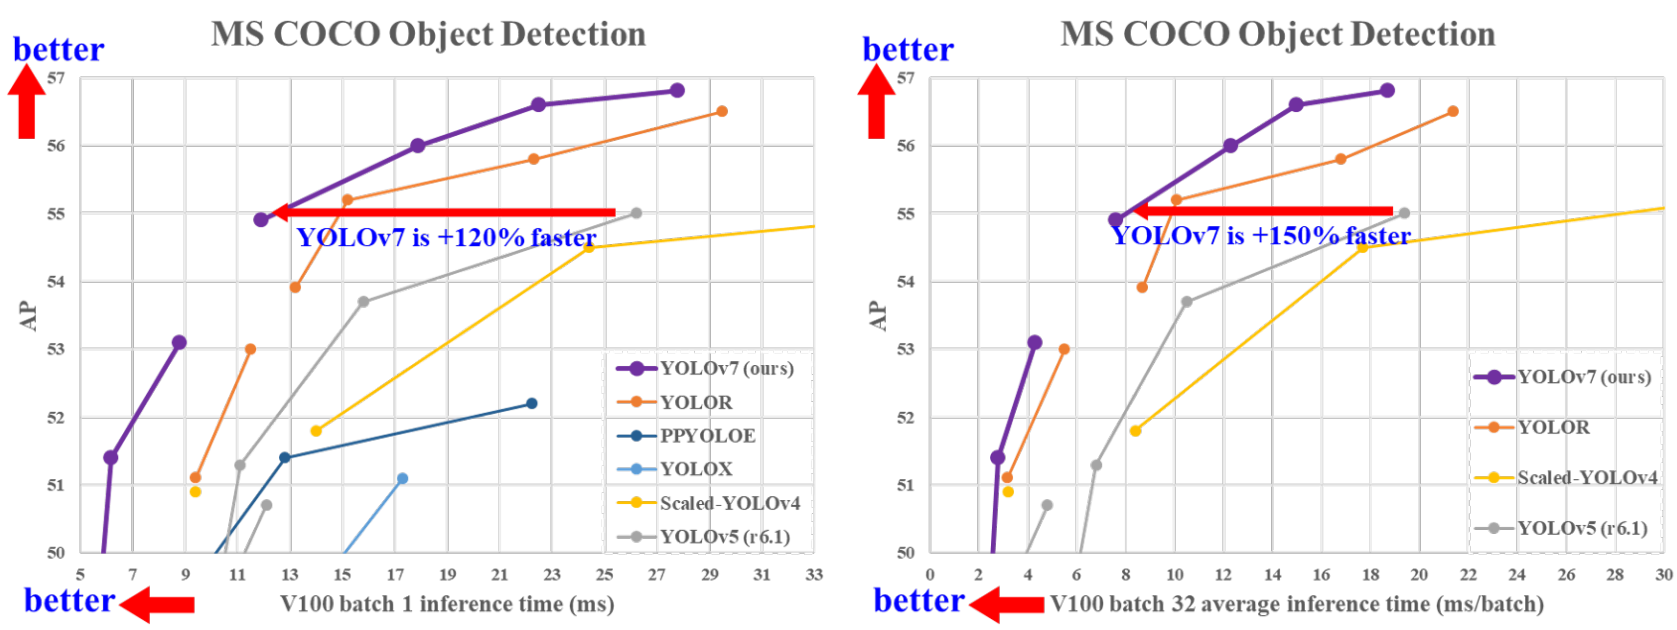
\includegraphics[width=\textwidth]{yolov7-performance.png}
	\caption{So sánh hiệu suất của Yolov7 và các real-time detector khác \textmd{(Ảnh trích xuất từ bài báo \citep{wang2022yolov7})}}
\end{figure}

YOLOv7 vượt qua mọi mô hình phát hiện đối tượng và các phiên bản YOLO trước đó trong cả tốc độ và độ chính xác trong khoảng từ 5 FPS đến 160 FPS và có độ chính xác cao nhất với 56.8\% AP trong số toàn bộ các mô hình phát hiện đối tượng hiện có, trong khi vẫn giữ được tốc độ 30 FPS hoặc nhiều hơn trên GPU V100. Bên cạnh đó, YOLOv7 yêu cầu phần cứng thấp hơn các mạng neural khác và có thể được huấn luyện nhanh hơn trên các dataset nhỏ mà không cần sử dụng bất kỳ pre-trained nào.

\subsection{Kiến trúc}
Một trong những cải tiến của YOLOv7 là thay đổi hàm kích hoạt (activation function) từ Leaky ReLU \cite{maas2013rectifier} sang Swish \cite{ramachandran2017searching} - một hàm kích hoạt mới hơn, có độ chính xác cao hơn và thời gian huấn luyện nhanh hơn so với Leaky ReLU. Các module cơ bản khác được tối ưu hóa dựa trên ý tưởng thiết kế của residual connection \cite{he2016deep}, nhưng kiến trúc cơ bản của không có nhiều sự thay đổi và vẫn bao gồm bốn phần chính, là: Input, Backbone, Neck và 	Prediction (Head).

\begin{figure}[h]
	\center
	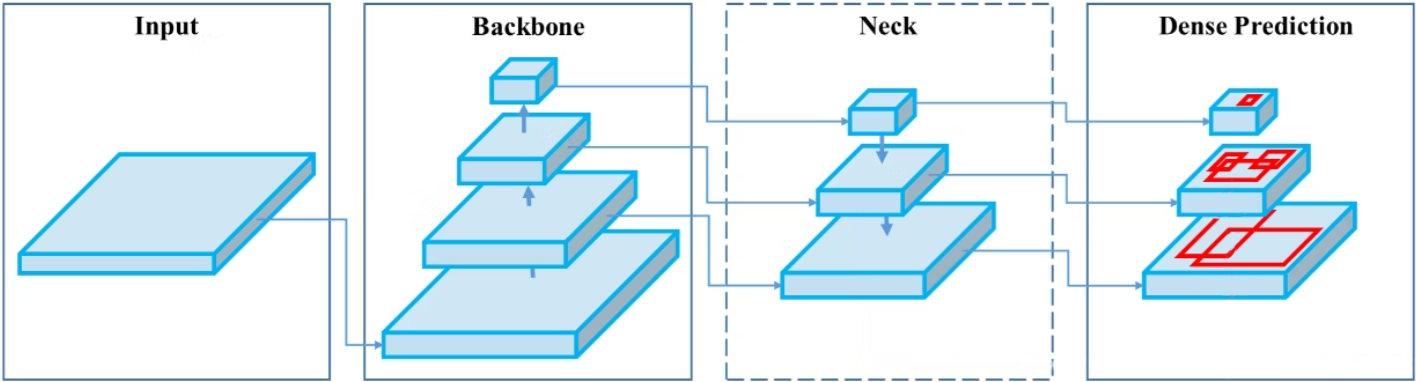
\includegraphics[width=\textwidth]{yolov7-architecture.png}
	\caption{Hình ảnh minh họa kiến trúc One-stage detector}
\end{figure}

\subsubsection*{Input}
Trong giai đoạn tiền xử lý, mô hình YOLOv7 áp dụng cả các kỹ thuật tăng cường dữ liệu \citep{bochkovskiy2020yolov4, tan2019mixconv}, đồng thời khai thác phương pháp tính toán anchor thích ứng (adaptive anchor) được thiết lập bởi YOLOv5 \cite{Glenn2022yolov5}, đảm bảo rằng các hình ảnh đầu vào được scale về tỷ lệ $640 \times 640$, đáp ứng yêu cầu về kích thước đầu vào của mạng Backbone.

\subsubsection*{Backbone}
Mạng Backbone đóng vai trò quan trọng nhằm trích xuất các đặc trưng.
Mạng Backbone cơ bản của các thuật toán YOLO là Darknet \cite{Redmon_2016_CVPR}, được xây dựng bởi Joseph Redmon vào năm 2016. Các phiên bản YOLO khác nhau tối ưu hóa mạng Darknet này theo các cách khác nhau, phụ thuộc vào kiến trúc của chúng. Mạng Backbone của YOLOv7 được cấu hình bao gồm ba thành phần chính: CBS (kết hợp giữa Convolution, Batch-norm và hàm kích hoạt SiLU), Extended-ELAN (E-ELAN) và MP1. Module E-ELAN cải thiện khả năng học của mạng bằng cách hướng các khối tính toán đặc trưng khác nhau để học được nhiều đặc trưng đa dạng hơn, trong khi vẫn giữ nguyên kiến trúc ELAN ban đầu và đường gradient gốc. Thành phần MaxPool-1 (MP1) bao gồm CBS và MaxPool, được chia thành nhánh trên và nhánh dưới. MaxPool trích xuất thông tin mang giá trị lớn nhất của các vùng địa phương (local) trong khi CBS trích xuất tất cả các thông tin về giá trị của các vùng địa phương, từ đó nâng cao khả năng trích xuất đặc trưng của mạng.

\subsubsection*{Neck (Feature Fusion Zone)} 
Lớp hợp nhất đặc trưng (feature fusion) được thiết kế nhằm cung cấp khả năng học tốt hơn các đặc trưng được trích xuất từ mạng Backbone. Các đặc trưng của các mức độ chi tiết khác nhau được học độc lập với nhau tại mạng Backbone và sau đó được hợp nhất tại lớp Neck của mạng, nhằm học được nhiều đặc trưng nhất có thể.

Mạng Neck của YOLOv7 được cấu trúc bằng kiến trúc Feature Pyramid Network (FPN)\cite{lin2017feature}, dựa trên thiết kế PANet \cite{Liu2018}. Mạng này bao gồm các CBS, cùng với cấu trúc Spatial Pyramid Pooling and Convolutional Spatial Pyramid Pooling (bao gồm hai mạng là SPPnet và CSPnet) \cite{he2015spatial, wang2020cspnet}, cùng với mạng E-ELAN và MaxPool-2 (MP2).  

\subsubsection*{Dense Prediction}
Áp dụng những ưu điểm của các thuật toán trước, YOLOv7 vẫn giữ lại ba detection heads. Các detection heads này được sử dụng để phát hiện đối tượng, đồng thời trả về xác suất dựa đoán (confidence score) và tọa độ khung dự đoán của đối tượng đó.

Mạng dự đoán của YOLOv7 sử dụng kiến trúc Rep, lấy cảm hứng từ RepVGG \cite{ding2021repvgg} và giới thiệu thiết kế residual đặc biệt nhằm hỗ trợ quá trình học của mạng. Thiết kế residual có thể đơn giản hóa thành một mạng tích chập trong các dự đoán thực tế, từ đó giảm độ phức tạp của mạng mà không ảnh hưởn đến độ chính xác dự đoán. Các đặc trưng từ tầng Neck được đưa qua mạng Rep để điều chỉnh số kênh ảnh, sau đó được áp dụng một tích chập để dự đoán độ tin cậy, loại vật thể và anchor.


\subsection{Trainable bag-of-freebies}
Bag-of-freebies (BoF) là một thuật ngữ được sử dụng trong lĩnh vực Machine Learning và Thị giác Máy tính. BoF bao gồm các kỹ thuật tiền xử lý hoặc tăng cường dữ liệu nhằm tăng cường hiệu suất mà không làm tăng độ phức tạp của mô hình. Trong họ YOLO, BoF lần đầu tiên được đề cập đến trong YOLOv4 \cite{bochkovskiy2020yolov4}. 
